% !TeX spellcheck = de_DE
\documentclass{alex_hü}

\name{Alexander Helbok}
\course{PS Physik}
\hwnumber{2}


\begin{document}
\renewcommand{\labelenumi}{\alph{enumi})}


\begin{mybox}{Materiewellen und Formfaktoren}
	\centering \(  \)
	\tcblower
	\begin{enumerate}
		\item \( R_{\text{Atom}} \approx 1.73 \unit{\angstrom};\quad R_{\text{Kern}} \approx 7.5 \unit{fm} \)
		\begin{flalign*}
 			\lambda_{\text{Atom}} &= \tfrac{h}{\sqrt{2E_{\text{Atom}}m_\alpha}} \stackrel{!}{=} R_{\text{Atom}} 
 				\quad\Rightarrow\quad E_{\text{Atom}} = \tfrac{2m_\alpha R_{\text{Atom}}^2}{h^2} 
 				= \dl{0.007 \unit{eV}} &&\\[1em]
% 				
 			\lambda_{\text{Kern}} &= \tfrac{h}{\sqrt{2E_{\text{Kern}}m_\alpha}} \stackrel{!}{=} R_{\text{Kern}}
 				\quad\Rightarrow\quad E_{\text{Kern}} = \tfrac{2m_\alpha R_{\text{Kern}}^2}{h^2} 
 				= \dl{3.67 \unit{MeV}} &&
		\end{flalign*}
	\tcbline
		\item \(  \)
		\begin{flalign*}
			F(\vec{q}^2) &= \uint[\mathbb{R}^3]{\expo[\iu\vec{q}\vec{x} / \hbar] f(\vec{x}) }{\vec{x}} 
				= \uint[0,2\pi]{\uint[0,\pi]{\uint[0,\infty]{\expo[\iu qr\cos(\theta) / \hbar] f(r) r^2 \sin(\theta)}{r}}{\theta}}{\varphi} &&\\
				&= 2\pi \uint[0,\infty]{f(r)r^2 \uint[0,\pi]{\expo[\iu qr\cos(\theta) / \hbar] \sin(\theta) }{\theta}}{r} 
				= 2\pi \uint[0,\infty]{f(r)r^2 \uint[-1,1]{\expo[\iu qru / \hbar] }{u}}{r} &&\\
				&= 4\pi \uint[0,\infty]{f(r)r^2 \left( \expo[\iu qr / \hbar] - \expo[-][\iu qr / \hbar] \right) \tfrac{\hbar}{2\iu qr}}{r}
				= 4\pi \uint[0,\infty]{\tfrac{\sin(\tfrac{qr}{\hbar})}{\tfrac{qr}{\hbar}} f(r)r^2}{r} &&
		\end{flalign*}
	\tcbline
		\item \( \langle r^2 \rangle = 4\pi\uint[0,\infty]{r^4f(r)}{r};\quad \tfrac{\sin(\tfrac{qr}{\hbar})}{\tfrac{qr}{\hbar}} \approx 1 + \tfrac{r^2q^2}{6\hbar^2} \)
		\begin{flalign*}
			F(\vec{q}^2) &\approx 4\pi \uint[0,\infty]{f(r) \left(r^2 + \tfrac{r^4q^2}{6\hbar^2} \right)}{r} 
				= 4\pi \uint[0,\infty]{f(r)r^2}{r} + \langle r^2 \rangle \tfrac{6\hbar^2}{q^2} 
				= 1 + \langle r^2 \rangle \tfrac{6\hbar^2}{q^2} &&\\[1em]
			&\Rightarrow \langle r^2 \rangle = \dl{\left( F(\vec{q}^2) - 1 \right)\tfrac{q^2}{6\hbar^2}} &&
		\end{flalign*}
	\tcbline
		\item \( f(r) = f_0\expo[-][ar] \)
		\begin{flalign*}
			\uint[\mathbb{R}^3]{f(\vec{x})}{\vec{x}} \stackrel{!}{=} 1 
				\quad\Longleftrightarrow\quad \uint[0,\infty]{f_0\expo[-][ar]r^2}{r} = \frac{1}{4\pi} 
				\quad\Longleftrightarrow\quad \dl{f_0 = \frac{a^3}{8\pi}} &&
		\end{flalign*}
	\tcbline
		\item \( F(\vec{q}^2) = \left(1+\alpha^2\right)^{-2} \)
		\begin{flalign*}
			F(\vec{q}^2) &= 4\pi \uint[0,\infty]{\tfrac{\sin(\tfrac{qr}{\hbar})}{\tfrac{qr}{\hbar}} f(r)r^2}{r} 
				= \frac{\hbar a^3}{2q} \uint[0,\infty]{\sin(\tfrac{qr}{\hbar}) \expo[-][ar] r}{r} 
				= \frac{a^4\hbar^4}{\left( a^2\hbar^2 + q^2 \right)^2} &&\\
			&\Rightarrow \alpha(q, a) = \dl{\frac{q}{a\hbar}} &&
		\end{flalign*}
		Diese Ladungsverteilung beschreibt Protonen.
	\tcbline
		\item \( f(r) = \begin{cases}
			\tfrac{3}{4\pi R_0^3} \quad &\text{für } 0 \leq r \leq R_0 \\
			0 \quad &\text{für }  R_0 < r
		\end{cases} \)
		\begin{flalign*}
				F(\vec{q}^2) &= 4\pi \uint[0,\infty]{\tfrac{\sin(\tfrac{qr}{\hbar})}{\tfrac{qr}{\hbar}} f(r)r^2}{r} 
					= 3\frac{\hbar}{qR_0^3} \uint[0,R_0]{\sin(\tfrac{qr}{\hbar}) r}{r} = &&\\
					&= 3\frac{\sin \left(\frac{qR_0}{\hbar}\right)- \tfrac{qR_0}{\hbar} \cos \left(\frac{qR_0}{\hbar}\right)}{\tfrac{q^3R_0^3}{\hbar^3}} 
					= 3\frac{\sin(x)- x\cos(x)}{x^3} \qquad, \text{mit } x(q) = \tfrac{qR_0}{\hbar}&&
		\end{flalign*}
		Diese Ladungsverteilung wird in der Natur nicht wiedergefunden, man kann schwerere Kerne aber dadurch approximieren.
	\tcbline
		\item \( x(0) = 0 \)
		\begin{flalign*}
			F(0) &= \lim_{x \to 0} \left(3\frac{\sin(x)- x\cos(x)}{x^3}\right)
				= 3\lim_{x \to 0} \left(\frac{1}{x^2}\right) 
				= \text{divergiert gegen }\infty && 
		\end{flalign*}
	\end{enumerate}
\end{mybox}

\begin{mybox}{Stabilstes Nuklid einer Isobare}
	 \( M(A,Z) = Z(m_\mathrm{P} + m_\mathrm{e}) + (A-Z)m_\mathrm{N} \newline \phantom{\hspace{2cm}} - ( a_{\text{V}}A - a_{\text{S}}A^{2/3} - a_{\text{C}}Z^2A^{-1/3} - a_{\text{A}}\tfrac{(A-2Z)^2}{A} + \delta a_{\text{P}} A^{-1/2})c^{-2} \)
	\tcblower
	\begin{enumerate}
		\item \(  \)
		\begin{flalign*}
			\pdv{M(A,Z)}{Z} &= m_{\text{P}} + m_{\text{e}} - m_{\text{N}} - \left( \tfrac{4a_{\text{A}}(A-2Z)}{A} - \tfrac{2a_{\text{C}}Z}{A^{1/3}}\right)c^{-2} 
				\stackrel{!}{=} 0 &&\\[1em]
			\Rightarrow Z_0(A) &= \frac{4a_A - (m_{\text{P}} + m_{\text{e}} - m_{\text{N}})c^2}{2A^{-1/3}(a_{\text{C}} + 4a_{\text{A}}A^{-2/3})} &&
		\end{flalign*}
	\tcbline
		\item \(  \)
			\begin{align*}
				Z_0(67) = 29.9979 \approx \dl{30} \qquad
					Z_0(118) = 50.2517 \approx \dl{50} 
			\end{align*}
			\begin{minipage}{\textwidth}
				\vspace{0cm}\hspace{0cm}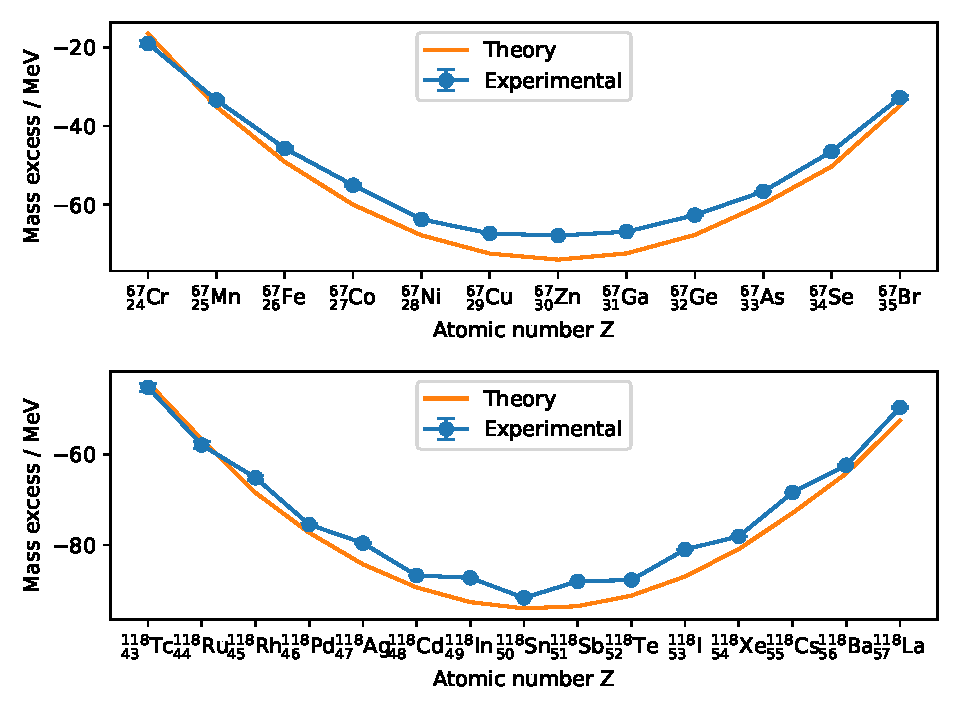
\includegraphics[width=0.9\textwidth]{plot1.pdf}
			\end{minipage}	
	\end{enumerate}
\end{mybox}

\begin{mybox}{Luminosität des LHC}
	\centering \(  \)
	\tcblower
	\begin{enumerate}
		\item \( \sigma = 0.07 \unit{\barn};\quad L_{\text{int}} \approx 200 \unit{\per\femto\barn} \)
		\begin{flalign*}
			L_{\text{int}} &= \uint[]{\frac{1}{\sigma}\dv{N}{t}}{t} = \frac{N}{\sigma} &&\\[2ex]
			\Rightarrow N &= L_{\text{int}}\sigma = \dl{1.4 \times 10^{16}} &&
 		\end{flalign*}
	\tcbline
		\item 
		\begin{itemize}[label=-]
			\item Die meisten pp-Wechselwirkungen fanden 2018 statt. 
			\item Die integrierte Luminosität kann mit der Zeit nicht abnehmen, da weder die Targetanzahl \( N \), noch der Fluss \( \phi \) negativ werden und daher die zu integrierende Funktion strikt positiv ist.
			\item Der LHC läuft nicht durchgehend, was die Sattelpunkte in den Graphen erklärt. Zudem werden unterschiedliche Kollisionsexperimente durchgeführt (p-p, p-Pb, Pb-Pb), welche mit unterschiedlichen Targets und Flüssen arbeiten.
		\end{itemize}
	\end{enumerate}
\end{mybox}


\end{document}